\documentclass[a4paper, fontsize=14pt]{article} \usepackage{course_work} \bibliography{course_work.bib}
%\usepackage{graphs/gnuplot-lua-tikz}
%\setcounter{page}{4} %в зависимости от того, какой по счёту страницей должно быть оглавление!

\begin{document}
%\includepdf[pages=-]{title-pages.pdf}
\newpage
\tableofcontents
\newpage
\section*{Введение}
\addcontentsline{toc}{section}{Введение}
К гиперболическим уравнениям приводят задачи колебания струны, движения сжимаемого газа,
распространения возмущения электромагнитных полей и многие другие.
% TODO написать еще что-нибудь

Целью данной курсовой работы является изучение распространения акустических волн в неоднородной
среде. Для достижения данной цели были поставлены следующие задачи:
\begin{enumerate}
    \item Изучить литературу по теме "Двухслойная акустическая схема для задачи распространения волн"
    \item Разработать программу для численного решения волнового уравнения в неоднородной среде.
    \item Проанализировать поведение волны на границе сред с разной акустической плотностью.
\end{enumerate}
\newpage
\section{Двухслойная акустическая схема}
\subsection{Одномерная акустическая схема для плоских акустических волн}
Плоские акустические волны описывает уравнение малых колебаний струны при наличии внешнего силового
поля $f$.
\begin{equation}
    \label{strEq}
    \begin{cases}
        \diff[2]{P}{t} = c^2 \diff[2]{P}{x} + f(x,t)\\
        \subs{t=0}{P} = \mu_1(x)\\
        \subs{t=0}{\diff{P}{t}} = \mu_2(x)\\
        \subs{x=0}{P} = \mu_3(t)\\
        \subs{x=a}{P} = \mu_4(t)\\
    \end{cases}
\end{equation}
Заменим уравнение \ref{strEq} второго порядка системой уравнений первого порядка. Введем потенциалы скоростей и
правой части.
\begin{gather*}
    V(x,t) = \int \limits_0^x \diff{P(\xi,t)}{t} \,d\xi\\
    F(x,t) = \int \limits_0^x f(\xi,t) \,d\xi
\end{gather*}
Тогда функции $P(x,t)$,$V(x,t)$ удовлетворяют системе уравнений \ref{acousticSys}. 
\begin{equation}
    \label{acousticSys}
    \begin{cases}
        \diff{P}{t} = \diff{V}{x}\\
        \diff{V}{t} = c^2 \diff{P}{x} + F(x,t)\\
        \subs{t=0}{P} = \mu_1(x)\\
        \subs{t=0}{V} = \int \limits_0^x \mu_2(\xi) \,d\xi\\
        \subs{x=0}{P} = \mu_3(t)\\
        \subs{x=a}{P} = \mu_4(t)\\
    \end{cases}
\end{equation}

Рассмотрим значения скоростей и давления в узлах равномерной пространственной и временной сеток
сеточных функций 
\begin{gather*}
    \omega_h =\{ih, i=\overline{0..N}\} \\ 
    \omega_\tau =\{i\tau,i=\overline{0..M},\tau = \frac{T}{M}\}\\
    y_i = P(x_i,t), x_i \in \omega_h\\
    \hat{y}_i = P(x_i,t+\tau), x_i \in \omega_h\\
    z_i = V\left(x_i+\frac{h}{2},t\right), i \leq N-1,x_i\in \omega_h\\
    \hat{z}_i = V\left(x_i+\frac{h}{2},t+\tau\right), i \leq N-1,x_i\in \omega_h\\
\end{gather*}

Составим явную акустическую схему, используя шаблон, изображенный на рисунке \ref{acousticTpl}.
\begin{figure}[h]
    \label{acousticTpl}
    \centering
    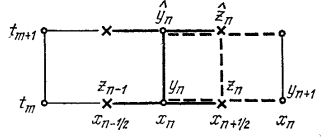
\includegraphics{scheme1d}
    \caption{шаблон одномерной акустической схемы}
\end{figure}
\begin{equation}
    \label{acousticScheme}
    \begin{gathered}
        \frac{\hat{z}_i - z_i}{\tau}=\frac{c^2}{h} (y_{i+1} - y_{i}) + F^{m+1/2}_{i+1/2}, 0\leq i\leq N-1\\
        \frac{\hat{y}_i - y_i}{\tau}=\frac{1}{h}(\hat{z}_i - \hat{z}_{i-1}), 1 \leq i \leq N-1
    \end{gathered}
\end{equation}
При выполнении условия Куранта $c\tau<h$ акустическая схема \ref{acousticScheme} сходится со
скоростью $O(h^2+\tau^2)$  \cite{kal}
\subsection{Двухмерная акустическая схема}


\cite{ufdtd}

\section{PML}
\cite{npml}

\newpage

\addcontentsline{toc}{section}{Список литературы}

\printbibliography


\end{document}
